\documentclass[aps,prb,onecolumn, footinbib, 10pt]{revtex4-2} 


\synctex=1 


\usepackage{amsmath,amssymb,bm} 
\usepackage{graphicx,comment}

\usepackage[tight]{subfigure} 

\usepackage[dvipsnames]{xcolor} 
\usepackage[papersize={8.5in,11in}]{geometry}
\usepackage[colorlinks=true]{hyperref}
\hypersetup{
    bookmarks=true,         % show bookmarks bar?
    unicode=false,          % non-Latin characters 
    pdftoolbar=true,        % show Acrobat
    pdfmenubar=true,        % show Acrobat 
    pdffitwindow=false,     % window fit to page when opened
    pdfstartview={FitH},    % fits the width of the page to the window
    pdfkeywords={keyword1} {key2} {key3}, % list of keywords
    pdfnewwindow=true,      % links in new window
    colorlinks=true,       % false: boxed links; true: colored links
    linkcolor=magenta, %red,          % color of internal links (change box color with linkbordercolor)
    citecolor=blue,        % color of links to bibliography
    filecolor=magenta,      % color of file links
    urlcolor=blue           % color of external links
} 

\geometry{top=1.5cm, left= 1.5 cm, right= 1.5 cm, bottom= 1.5 cm}        



%========================= PACKAGES ==================================
\usepackage{graphicx}
\usepackage{dcolumn}
\usepackage{color}
\usepackage{amssymb,amsmath, makecell}
\usepackage{tabularx, graphicx}
\usepackage{epstopdf}
\usepackage{latexsym}
\usepackage{colortbl}
\usepackage{psfrag}
\usepackage{bbm,bm,array,physics}
\usepackage{dsfont}
\usepackage{float, mathrsfs}

\def \nn{\nonumber \\}
\newcommand{\bs}[1]{\boldsymbol{#1}}



%=======================================================================
\begin{document}
\title{Direction-dependent conductivity for vortex nodal-rings}

\author{Fasil Hussain Rather}
\author{Ipsita Mandal}
\email{ipsita.mandal@snu.edu.in}

\affiliation{Department of Physics, Shiv Nadar Institution of Eminence (SNIoE), Gautam Buddha Nagar, Uttar Pradesh 201314, India}


\begin{abstract}
We focus on deriving the transport characteristics unique to two-band semimetals hosting nodal curves in the form of rings and featuring a smoke-ring like pseudospin structure. Dubbed as vortex nodal-ring (VNR), they inherently host nonzero vector fields of Berry curvature and orbital magnetic moment in the Brillouin zone, which endow it with longitudinal and planar-Hall magnetoelectric conductivity ($\bs \sigma$), analogous to topological nodal points. Continuing with our efforts to elucidate the fingerprints of different semimetals, we embark on analysing distinct configurations resulting from the relative orientation of the VNR's plane with respect to the plane defined by the applied electric ($\bs E $) and magnetic ($\bs B$) fields. We chalk out a holistic description of all the nonzero components of $\bs \sigma $, taking into account the Drude, anomalous-Hall, longitudinal, and transverse currents.
\end{abstract}

\maketitle

 \tableofcontents

% keywords: ideal gapped nodal-ring; electromagnetic fields in planar-Hall configurations; Berry curvature and orbital magnetic moment; anomalous-Hall effect effect; Lorentz-force-operator and its contributions

%irrefutable

%========================= BODY OF THE ARTICLE =========================
\section{Introduction}

Investigations of transport properties in three-dimensional (3d) semimetals have catapulted into prominence as they often reflect the underlying topological features of the Brillouin zone (BZ). When the BZ harbours symmetry-protected band-crossings in the momentum space (denoted here by $\bs k \equiv \lbrace k_x, k_y, k_z \rbrace $), the resulting nodal points~\cite{burkov11_Weyl, yan17_topological, bernevig, grushin-multifold} or curves~\cite{balents-nodal, vortex-nrsm} can be characterised by some topological invariant or index. Our efforts are mainly directed at identifying meaningful response which will capture this invariant unambiguously.
The topological properties often arise as a nontrivial Berry curvature (BC)~\cite{xiao_review, *sundaram99_wavepacket,graf-Nband, *graf_thesis}, sourced by the Berry phases of the associated Bloch bands meeting at the nodes of a semimetal. Starting with the pioneering example of the Weyl semimetals (WSMs), the most important telltale signatures of the BC are the intrinsic anomalous-Hall effect~\cite{haldane04_berry,goswami13_axionic, burkov14_anomolous} and the appearance of longitudinal and transverse conductivity in planar-Hall configurations \cite{zhang16_linear, chen16_thermoelectric, nandy_2017_chiral, *nandy18_Berry, *ips-mwsm-floquet, amit_magneto, *das20_thermal, ips-kush-review, ips-ruiz, *ips-tilted, ips-rsw-ph, *ips-shreya, ips-spin1-ph, timm, *ips-exact-spin1, *ips-exact-kwn, * ips-exact-rsw, phe_nlsm, ips-nlsm-ph, *ips-exact-kwn}. Here, we will focus on a two-band system containing a nodal-loop in the form of a circle [see Fig.~\ref{figfs}(a)], thus carrying a representation of the pseudospin-1/2 quantum number (just like the WSMs). Generically, their effective Hamiltonian can be represented as $\boldsymbol{d} (\bm k) \cdot \boldsymbol \sigma$, where $ \boldsymbol{\sigma} = \left\lbrace \sigma_x,\sigma_y,\sigma_z\right \rbrace $ is the vector comprising the three Pauli matrices as its three components and defining the $2\times 2$ matrix-operators in the pseudospin space. The 3-component vector $\bs d$ encodes the pseudospin structure of the two-component spinors representing the two Bloch bands. For a typical nodal-loop protected by $\mathcal P \mathcal T$-symmetry (where $\mathcal P$ and $\mathcal T$ represent the operators implementing the inversion and time-reversal symmetries, respectively), has a nonzero BC only along the loop itself, vanishing identically elsewhere
%%%%%%%%%%%
\footnote{Adding a mass term of magntitude $\Delta $, for example generated by spin-orbit coupling, makes it gapped. This induces a nonvanishing BC $\propto \Delta$ which happens to have only in-plane components \cite{schnyder_nodal, yang1, yang_review_nlsm, chen_nlsm, ips-magnus, flores, phe_nlsm, claudia_nlsm, enke, ips-nlsm-ph}.}.
%%%%%%%%%%%%%%
This singular-natured BC is characterised by a nonvanishing Zak phase \cite{schnyder_nodal, biao_nodal, zak_nodal, ips-nlsm-ph}. However, in the absence of both these symmetries, a different type of nodal-ring may exist, dubbed as the vortex nodal-ring (VNR) \cite{vortex-nrsm}, which does harbour a nonvanishing nonsingular BC away from the nodal-loop. The nomenclature is related to the fact that the vector field representing $\boldsymbol d (\bf k)$ takes a vortex-like or smoke-ring texture in the momentum space [cf. Fig.~\ref{figfs}(b)]. For the ease of reference, we will refer to the other variety of nodal-ring and its gapped cousins (obtained by starting from the $\mathcal P \mathcal T$-symmetric model) as the non-vortex nodal-ring (NVNR).


The BC is accompanied by another vector field called the orbital magnetic moment (OMM), sourced by the same Berry phase \cite{xiao_review,*sundaram99_wavepacket}, and also affects transport involving a magnetic field \cite{ips-ruiz, *ips-tilted, ips-rsw-ph, *ips-shreya, ips-spin1-ph, ips-exact-spin1, *ips-exact-kwn, * ips-exact-rsw, ips-nlsm-ph}. While topology-induced response has been studied quite widely for the NVNRs \cite{schnyder_nodal, yang1, yang_review_nlsm, chen_nlsm, ips-magnus, flores, phe_nlsm, claudia_nlsm, enke, ips-nlsm-ph}, such characteristics have not explored for the VNRs, which are the systems of interest in this paper. In particular, we will perform an analytical computation of the linear magnetoelectric conductivity in planar-Hall set-ups, similar to what was studied in our earlier work involving NVNRs \cite{ips-nlsm-ph}. Such set-ups refer to the application of static and uniform electric ($\bs E $) and magnetic ($\bs B$) fields, where $\bs B $ is not necessarily perpendicular to $\bs E $. The most intriguing feature to probe is the nature of an emergent in-plane conductivity, which is caused by the BC and the OMM. The word in-plane refers to the $\bs E \bs B$-plane. Since the VNR's plane gives us another direction to play around with, the relative orientations of these two planes, in fact, allow us to define distinct planar-Hall set-ups. Similar situations are encountered for other semimetals with anisotropic dispersions \cite{ips-tilted, rahul-jpcm}.

The paper is organized as follows. In Sec.~\ref{secmodel}, we explain the form of the effective Hamiltonian for a VNR. Sec.~\ref{secsigma} contains the details of computation and final results for the various components of the magnetoelectric conductivity. We elucidate the significant differences between VNRs and NVNRs in Sec.~\ref{seccompare}. A tilt term (of strength $\eta$) with respect to any direction along the nodal plane can cause the toric Fermi surface (in the untilted case) to deform into cyclides of various types (e.g., horn- and spindle-cyclides) \cite{ahn-tilted-nl}. Accordingly, the corresponding variation of conductivity is derived and discussed in \ref{sectilt}. Finally, we conclude by summarising our findings in Sec.~\ref{secsum}, supplemented by some future perspectives. 


All our expressions in the paper are written using the natural units. Basically, this implies that the reduced Planck's constant ($\hbar $), the speed of light ($c$), and the Boltzmann constant ($k_B $) are each set to unity. The magnitude of electric charge, $e$, has no units and also equals unity in the natural units. However, for tracking the appearance of the electric charge, we will retain $e$ in our expressions. 


%%%%%%%%%%%%%%%%%%%%%%%%%%
\section{Model}
\label{secmodel}


%%%%%%%%%%%%%%%%%%%%%%%%%%%%%%%%%%%%%%%%%%%%%%%%%%%%%%%%%
\begin{figure*}[t]
\subfigure[]{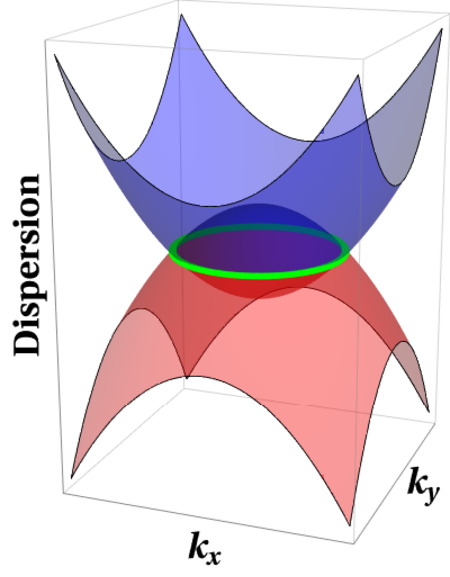
\includegraphics[width=0.23 \textwidth]{disp-vr}} \hspace{ 1 cm}
\subfigure[]{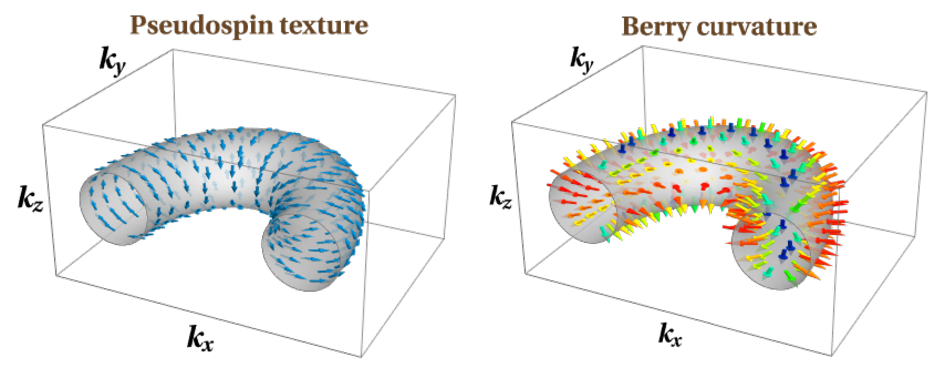
\includegraphics[width=0.65 \textwidth]{spin-Om}  }
\caption{\label{figfs} Pictorial depiction of some unique features of a VNR:
(a) Dispersion against the $k_x k_y $-plane showing two bands crossing along a circle (highlighted in green), setting $k_z = 0 $. (b) Nature of the vector fields ${\bs d} (\bs k)$ [or, equivalently, ${\bs d}_0 (\bs k)$ in the vicinity of the VNR] and $\bs \Omega_{s=2} (\bs k)$ in the vicinity of a section of the toroidal Fermi surface (gray). The former displays a smoke-ring pattern.}
\end{figure*}
%%%%%%%%%%%%%%%%%%%%



The minimal model of a VRN, comprising two bands and a circular nodal-loop lying in the $k_x k_y$-plane at $k_z = 0$, is captured by \cite{vortex-nrsm}
%%%%%%%%%%%%%%%%%%%%%%%
\begin{align}
\mathcal{H}_0 (\bs k ) = {\bs d}_0 (\bs k) \cdot \boldsymbol{\sigma} \,,
\quad {\bs d}_0 (\bs k)
= \left \lbrace  \frac{-\,k_x\,k_z} {m_z}, \,\frac{-\,k_y\, k_z} {m_z},
\, \frac{ k_\perp^2-k_0^2 - k_z^2} {2\,m_\perp}  \right \rbrace, \quad
k_\perp = \sqrt{k_x^2 + k_y^2 }\,,
\end{align}
%%%%%%%%%%%%%%%%%%
where $k_0$, $m_z$, and $m_\perp $ are material-dependent parameters. At the $ k_z = 0$ plane, the two bands cross at $k_\perp = k_0  $, defining a nodal-ring of radius $ k_0 $. Therefore, $v_z \equiv k_0/m_z$ and $v_\perp \equiv k_0/m_\perp $ encode the values of the Fermi velocities perpendicular and parallel to the nodal plane, respectively. In the following, we will set $v_z = v_\perp  = v_0 $ for the sake of simplicity.


For low-energy excitations confined in the vicinity of the resulting Fermi surface, the dominant transport-signatures of the low-energy quasiparticles can be captured by a linearised Hamiltonian, $\mathcal{H}$. It comprises terms which deviate only at linear-order-in-momentum from the location of the nodal line \cite{linearize-nlsm, ips-nlsm-ph}. This can be accomplished by implementing a transformation to the cylindrical coordinates as follows:
\begin{align}
\label{eqtrs}
k_x = k_\perp \cos \phi \,, \quad
k_y = k_\perp \sin \phi \,,\quad k_\perp =  k_0 + \kappa_\perp \,.
\end{align}
%%%%%%%%%%%%%%%%%%%%%
Clearly, $ \kappa_\perp \in [-\, k_0,\,\infty )$. However, for the low-energy processes we are interested in, we must have $|\kappa_\perp | \ll k_0 $, as $k_0$ acts as an ultraviolet-energy scale.
Subsequently, linearising in the small-valued variables (viz. $\kappa_\perp $ and $k_z$), we end up with
% https://en.wikipedia.org/wiki/Torus#Geometry
%%%%%%%%%%%%%%%%%%%%%%%%
\begin{align}
\label{eqham}
& \mathcal{H} (\bs k) = {\bs d} ( \bs k) \cdot \boldsymbol{\sigma} \,,
\quad
{\bs d} ( \bs k) = v_0 \left \lbrace  - \,k_z \cos \phi,\,
-\,k_z \sin \phi,\, \kappa_\perp \right \rbrace.
\end{align}
%%%%%%%%%%%%%%%
For the linearised Hamiltonian $\mathcal H$, the eigenvalues of the two bands are obtained as
\begin{align}
\label{eqev}
\varepsilon_s  ({ \bs k}) &= (-1)^s\, \epsilon_k \,, \quad 
 \epsilon_k = v_0\, \sqrt{ \kappa_\perp^2 +  k_z^2}, 
\quad s \in \lbrace 1,2 \rbrace.
\end{align}
The band velocity of the quasiparticles is given by
\begin{align}
\label{eqv}
{\boldsymbol v}^{(0,s)} ( \bs{k}) 
\equiv \nabla_{\bs{k}} \varepsilon_s  (\bs{k})
%%%%%%%%
= \frac{ (-1)^s\, v_0^2}{\epsilon_k }  \left\lbrace 
\kappa_\perp \cos \phi, \, \kappa_\perp \sin\phi , \,k_z
\right\rbrace  .
\end{align}
%%%%%%%%%%%%%%%
The Berry curvature (BC) and the orbital magnetic moment (OMM), associated with the $s^{\rm{th}}$ band, turn out to be
\begin{align}
\label{eqbcomm}
\bs \Omega_s ({ \bs k})= 
\frac{(-1)^{s+1} \, v_0^3\,k_z} 
{2\, (k_0 + \kappa_\perp )\, \epsilon_k^3}
\left\lbrace \kappa_\perp \cos \phi  , \, \kappa_\perp \sin \phi,\, k_z \right\rbrace, \quad 
%%%%%%%%%%
{\boldsymbol{m}} ({ \bs k}) 
= \frac{ -\,e \, v_0^3\,k_z} 
{2\, (k_0 + \kappa_\perp )\, \epsilon_k^2}
\left\lbrace \kappa_\perp \cos \phi  , \, \kappa_\perp \sin \phi,\, k_z \right\rbrace.
\end{align}
%%%%%%%%%%
Therefore, the shift in energy caused by the OMM is captured by
\begin{align}
\varepsilon_m ({ \bs k}) 
= \frac{e \,v_0^3 \,k_z 
\left( B_x \,\kappa_\perp  \cos \phi + B_y \,\kappa_\perp  \sin \phi 
+ B_z k_z \right)}
{2 \,\epsilon_k^2 \,(k_0 + \kappa_\perp )}\,.
\end{align}
The OMM-induced parts are the same for both the bands and, hence, we have not attached any $s$ index to them.

For the ease of performing the integrals, it is useful to switch to the toroidal coordinates, where we define
\begin{align}
\label{eqtorus}
k_z = \kappa \sin \gamma \text{ and } \kappa_\perp = \kappa \cos \gamma\,, \text{ with } \gamma \in [0, \, 2\,\pi)\,.
\end{align}
Interpreted in terms of the toroidal coordinates, $k_0$ represents the major radius (i.e., the distance between the origin and a point on the node's circle) and $\kappa $ denotes the radius of the cross-section of the torus. 

%%%%%%%%%%%%%%%%%%%%%%%%%%%%%%%%%%%%%%%%%%%%%%%%%%%
\section{Magnetoelectric conductivity}
\label{secsigma}



%%%%%%%%%%%%%%%%%%%%%%%%%%%%%%%%%%%%%%%%%%%%%%%%%%%
\section{Comparison of the results with those for gapped NVNRs}
\label{seccompare}

For the gapped NVNR, since the BC and the OMM lacked any $z$-components, a major number of terms in the conductivity reduced to zero, which also led to the vanishing of certain components in set-ups II and III. Here, instead we find a richer structure, where such vanishing does not occur.


%%%%%%%%%%%%%%%%%%%%%%%%%%%%%%%%%%%%%%%%%%%%%%%%%%%
\section{For future: Effects of tilting on conductivity}
\label{sectilt}



%%%%%%%%%%%%%%%%%%%%%%%%
\begin{align}
\label{eqhamtilt}
& \mathcal{H}_t (\bs k) = {\bs d} ( \bs k) \cdot \boldsymbol{\sigma} + \eta \,v_0\, k_x\,\mathbb{I}_{2 \times 2}\,.
\end{align}
%%%%%%%%%%%%%%%
\begin{align}
\label{eqevt}
\varepsilon_s  ({ \bs k}) &= (-1)^s\, \epsilon_k + \eta \,v_0\, (k_0+\kappa_\perp) \cos \phi \,,
\quad {\boldsymbol v}^{(0,s)} ( \bs{k})  = \left\lbrace \eta + ...., \, ....,\,....\right\rbrace.
\end{align}
The tilting does not affect the BC and the OMM because the addition of a term $\propto \mathbb{I}_{2 \times 2}$ to the Hamiltonian cannot change the structure of the eigenvectors.


Since the rotational symmetry in the $xy$-plane is broken by the tilt term, we need to consider three more nonequivalent set-ups as follows:
\begin{itemize}

\item Set-up IV: $ \mathbf{E} = E_y\, {\mathbf{\hat y}}$ and $\mathbf{B} = B_x\,{\mathbf{\hat x}} + B_y\,{\mathbf{\hat y}}$.

\item Set-up V: $\mathbf{E} = E_y \,{\mathbf{\hat y}}$ and $ \mathbf{B} = B_x\,{\mathbf{\hat x}} + B_z \,{\mathbf{\hat z}} $.

\item Set-up VI: $\mathbf{E}= E_z\,{\mathbf{\hat z}}$ and $\mathbf{B} = B_y\,{\mathbf{\hat x}} + B_z \,{\mathbf{\hat z}}$.

\end{itemize}
%%%%%%%%%%%%%%%%%%%%%%%%
In the language of Eq.~\eqref{eqtorus}, we have $\epsilon_k =  v_0 \, \kappa $ and
\begin{align} 
&\delta (\varepsilon_s -\mu)  \equiv 
\delta \Big (  (-1)^s\,v_0 \,\kappa + \eta \,v_0\, (k_0 + \kappa \cos \gamma) \cos \phi -\mu \Big )
= \frac{\delta \Big ( \kappa - \frac{\mu - \tilde \eta \cos \phi } { v_0\,\zeta_s } \Big )}
{ v_0 \,|\zeta_s| } \,,
\nn & \text{where }
\zeta_s = (-1)^s  + \eta  \cos \gamma \cos \phi
\text{ and } \tilde \eta = \eta\,v_0\,k_0.
\end{align}
Depending on the relative values of $\mu$ and $ \tilde \eta $, both the bands may contribute, and the valid range of $\phi $ is determined from the points where the Fermi-momentum vanishes. The latter is determined from $\kappa = 0 \Rightarrow  \cos \phi  =  \mu /\tilde \eta $. 




%%%%%%%%%%%%%%%%%%%%%
\section{Summary and outlook}
\label{secsum}

A future direction will be to derive the explicit analytical description of the Fermi arcs, as has been done recently for nodal-point semimetals \cite{ips-fa}.





%%%%%%%%%%%%%%%%%%%%%%%%%%%%%%%%%%%%%

\bibliography{ref_nl} 


\end{document}






